\section{泛函优化问题}
\label{sec:func-problem}

当未知量是一个函数时，一个优化问题要写清哪些东西？我们从两个具体目标出发，先把它们看成很长的向量上的优化，再说明目标、函数空间和边界约束各自规定了什么。

\paragraph{两个目标}
考虑区间$[0,1]$上的函数$u$，要求它过两个固定端点：
\begin{equation}
 u(0)=0,\qquad u(1)=1.
 \label{eq:func-endpoints}
\end{equation}
第一个目标是曲线$y=u(x)$的长度：
\begin{equation}
 \ell(u)=\int_0^1\sqrt{1+u'(x)^2}\,\mathrm{d}x.
 \label{eq:func-length}
\end{equation}
第二个目标是一根细线的能量：
\begin{equation}
 E(u)=\int_0^1\Bigl(\frac12u'(x)^2+\frac12u(x)^2\Bigr)\,\mathrm{d}x.
 \label{eq:func-energy}
\end{equation}
$u'^2$一项惩罚倾斜，它希望曲线尽量平直；$u^2$一项是弹簧的拉力，它希望曲线靠近横轴。两端的约束又不许曲线贴着横轴走，最优形状是两者的折中。式~\eqref{eq:func-energy}将贯穿全章。

候选函数不同，这两个数也不同。对$u(x)=x$和$u(x)=x^2$逐项积分，得到
\[
 \ell(x)=\sqrt2\approx1.4142,\qquad \ell(x^2)=\frac{\sqrt5}{2}+\frac14\operatorname{arcsinh}2\approx1.4789,
\]
以及
\[
 E(x)=\frac12+\frac16=\frac23,\qquad E(x^2)=\frac23+\frac1{10}=\frac{23}{30}.
\]
直线在这两个目标下都比抛物线好。直线是不是这两个目标下的最好选择，现在还回答不了。

\paragraph{函数是很长的向量}
怎样把函数放进前面各章的框架？取$\Delta=1/n$，结点$x_i=i\Delta$，只记录结点高度$u_i=u(x_i)$，$i=0,\ldots,n$。图~\ref{fig:func-grid-vector}中的绿色竖线就是这些坐标。两端的$u_0=0$和$u_n=1$已被约束固定，自由的坐标是$u_1,\ldots,u_{n-1}$。

\begin{BookInlineFigure}
  \centering
  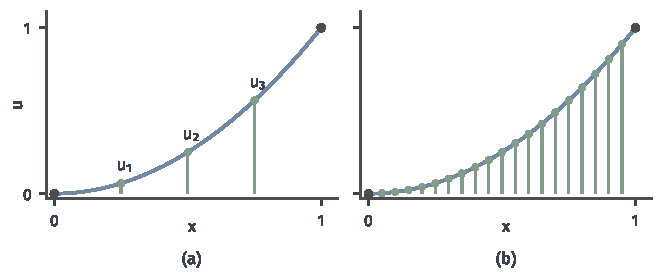
\includegraphics[width=112mm]{figures/05-optimization/08-functional-optimization/matplotlib/func-grid-vector/figure.pdf}
  \caption{函数$u(x)=x^2$的结点值。灰色点是被端点约束固定的值，绿色竖线是自由坐标。(a)$n=4$，自由坐标$u_1,u_2,u_3$。(b)$n=20$，自由坐标有$19$个。切得越细，向量越长，曲线的形状也记录得越完整。}
  \label{fig:func-grid-vector}
\end{BookInlineFigure}

用差商代替导数，用求和代替积分，式~\eqref{eq:func-energy}变成一个普通的多元函数。其中$u'^2$一项写成
\[
 \int_0^1\frac12u'(x)^2\,\mathrm{d}x\approx\sum_{i=0}^{n-1}\frac{\Delta}{2}\Bigl(\frac{u_{i+1}-u_i}{\Delta}\Bigr)^2
 =\frac{1}{2\Delta}\sum_{i=0}^{n-1}(u_{i+1}-u_i)^2.
\]
这是自由坐标的二次函数。取$n=2$，唯一的自由坐标是$u_1$。对$u^2$一项用梯形求积，得到一元二次函数
\[
 E_2(u_1)=u_1^2+(1-u_1)^2+\frac14u_1^2+\frac18.
\]
令导数$2u_1-2(1-u_1)+\frac12u_1$为零，解出$u_1=4/9\approx0.444$。这是用一个坐标对曲线中点高度的估计。

对应关系可以列成一张表，它只是起点，更多的对应要到后面几节才能建立。

\begin{BookInlineTable}
  \centering
  \caption{向量与函数的对应关系。}
  \label{tab:func-analogy}
  \begin{tabular}{ll}
    \toprule
    向量 $\bm{x}\in\mathbb{R}^n$ & 函数 $u$\\
    \midrule
    下标 $i$ & 位置 $x$\\
    坐标 $x_i$ & 取值 $u(x)$\\
    求和 $\sum_ix_iy_i$ & 积分 $\int u(x)v(x)\,\mathrm{d}x$\\
    目标函数 $f(\bm{x})$ & 目标泛函 $J(u)$\\
    线性约束的解集 & 固定边界值的函数集\\
    \bottomrule
  \end{tabular}
\end{BookInlineTable}

这个类比能直接告诉我们该问什么，却不能直接给出答案。$n$变大时维数没有上限，有限维里“维数固定”才成立的结论都要重新检查。

\paragraph{问题的写法}
有了具体例子，就可以写出一般形式。函数虽然被看成向量，写法上不加粗，可行集仍记作$\bm{C}$。

\begin{definition}[泛函优化问题]
\label{def:func-problem}
设$X$是实赋范空间，$\bm{C}\subseteq X$非空，$J:\bm{C}\to\mathbb{R}\cup\{+\infty\}$，且至少有一点取有限值。把输入函数、输出实数的$J$称为\term{目标泛函}（objective functional），问题
\begin{equation}
 \min_{u\in\bm{C}}J(u)
 \label{eq:func-problem}
\end{equation}
称为\term{泛函优化问题}（functional optimization problem）。记$J^\star=\inf_{u\in\bm{C}}J(u)$。若$u^\star\in\bm{C}$使$J(u^\star)=J^\star$，称$u^\star$为最优解。
\end{definition}

这里的\term{泛函}（functional）指定义在函数集合上、取值为数的映射。有限维问题只要写目标和约束，因为$\mathbb{R}^n$上的范数彼此等价，谈“附近”时不用说明用哪个范数。函数问题多出一项要写：空间$X$及其范数。它规定了三件事：哪些函数算候选，目标在哪里有限，两个函数怎样才算接近。

\paragraph{选择函数空间}
以$E$为例比较三个候选空间。若取$X=C^1[0,1]$，后面会看到极小化序列可能跑出这个空间；此外$E$用到的是导数的平方积分，它并不是$C^1$范数。若取$X=L^2(0,1)$，空间很大，但多数函数没有平方可积的导数，$E$只能取$+\infty$，端点值也没有意义，因为改变函数在一点的值不改变$L^2$中的元素。

合适的选择是让目标所用的量正好被范数控制，也就是取Sobolev空间
\begin{equation}
 H^1(0,1)=\bigl\{u\in L^2(0,1):u'\in L^2(0,1)\bigr\},\qquad
 \lVert u\rVert_{H^1}^2=\lVert u\rVert_2^2+\lVert u'\rVert_2^2.
 \label{eq:func-h1}
\end{equation}
其中$u'$是弱导数。$H^1(0,1)$是Hilbert空间，式~\eqref{eq:func-energy}的$E$恰好等于$\frac12\lVert u\rVert_{H^1}^2$。

下面要用到这个空间的三条性质。第一，每个$u\in H^1(0,1)$有连续代表，$u(y)-u(x)=\int_x^yu'(t)\,\mathrm{d}t$，所以端点值有意义。第二，点值受范数控制：
\begin{equation}
 \lvert u(y)\rvert\leq\sqrt2\,\lVert u\rVert_{H^1},\qquad y\in[0,1].
 \label{eq:func-point-bound}
\end{equation}
因此读取一点的值是$H^1(0,1)$上的连续线性泛函，在$L^2$中则不连续。第三，记端点为零的子空间为$H^1_0(0,1)$，其上有Poincaré不等式$\lVert v\rVert_2\leq\lVert v'\rVert_2$。这些结论的证明可参考\BookChapterRef{chap:sobolev-spaces}{卷四第21章“Sobolev空间”}。

\paragraph{允许怎样改变候选}
在$X=H^1(0,1)$中，端点条件~\eqref{eq:func-endpoints}给出可行集
\begin{equation}
 \bm{C}=\bigl\{u\in H^1(0,1):u(0)=0,\ u(1)=1\bigr\}.
 \label{eq:func-feasible}
\end{equation}
它不是线性子空间：两个可行函数的和在$x=1$处等于$2$。但两个可行函数的差在两端都为零。取$u_0(x)=x$，于是
\begin{equation}
 \bm{C}=u_0+\bm{V},\qquad \bm{V}=H^1_0(0,1).
 \label{eq:func-affine}
\end{equation}
这与线性方程组$\bm{A}\bm{x}=\bm{b}$的解集写成特解加零空间$\bm{x}_0+\operatorname{null}\bm{A}$完全相同。两个端点条件相当于两条线性约束，子空间$\bm{V}$只比$H^1(0,1)$少两个方向，但它仍是无限维的。

图~\ref{fig:func-feasible-directions}画了几个可行候选和它们与$u_0$的差。候选彼此差别很大，但(b)中所有的差都在两端归零。今后把这样的差称为扰动，记作$\eta$。求最优解时只能沿$\bm{V}$中的方向改变候选，这是第~\ref{sec:func-optimality}节最优性条件的出发点。

\begin{BookInlineFigure}
  \centering
  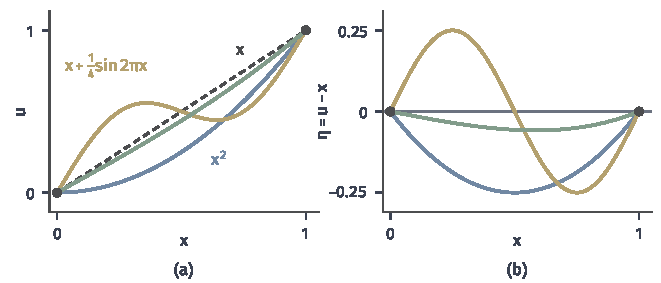
\includegraphics[width=112mm]{figures/05-optimization/08-functional-optimization/matplotlib/func-feasible-directions/figure.pdf}
  \caption{固定端点下的候选与扰动。(a)过$(0,0)$与$(1,1)$的候选：灰色虚线$u_0=x$、蓝色$x^2$、黄色$x+\frac14\sin2\pi x$，绿色是$\sinh x/\sinh1$。(b)同样颜色的三个差$\eta=u-x$，它们都在端点为零，属于方向子空间$\bm{V}=H^1_0(0,1)$。}
  \label{fig:func-feasible-directions}
\end{BookInlineFigure}

约束不同，允许的扰动也不同。若只固定$u(1)=1$而放开$u(0)$，扰动在$x=0$处可以取任意值，方向多了一个。若要求曲线处处不低于一个给定函数$\psi$，某些位置只能向上改动，能走的方向就依赖当前的候选。可行方向的这些差别，后面都会反映到最优性条件里。
